\documentclass{article}
\usepackage{graphicx}
\usepackage{float}
\usepackage{listings}
\usepackage{todonotes}
\usepackage[toc,page]{appendix}
%\usepackage[margin=1.5in]{geometry}

\begin{document}

\title{Virtual Power Plant design document}
\author{Ubbe Welling\\ubbe@eng.au.dk}

\maketitle
\begin{abstract}
The present paper documents the design phase of a new integrated Virtual Power Plant platform.
\end{abstract}



\setcounter{tocdepth}{2}
\tableofcontents

\section{Overview}
The purpose of the Virtual Power Plant (VPP) platform is to:
\begin{itemize}
	\item receive measurements from sensors deployed in a building.
	\item receive current and forecast information from external sources on grid load, electricity price and more.
	\item process measurements and external information to make decisions on power usage.
	\item actuate devices deployed in a building to implement abovementioned decisions.
\end{itemize} 

The platform will consist of one main server application with an attached database. 

\section{Database design}
The database will reside in a PostgreSQL DBMS.


\section{Application design}
The application will be programmed in object-oriented Python, using Python processes to enable concurrent processing.

Key classes have been identified to form a static structure which is shown in figure \ref{figureClassDiagram} and elaborated below:

\begin{figure}[H]
    \centering
    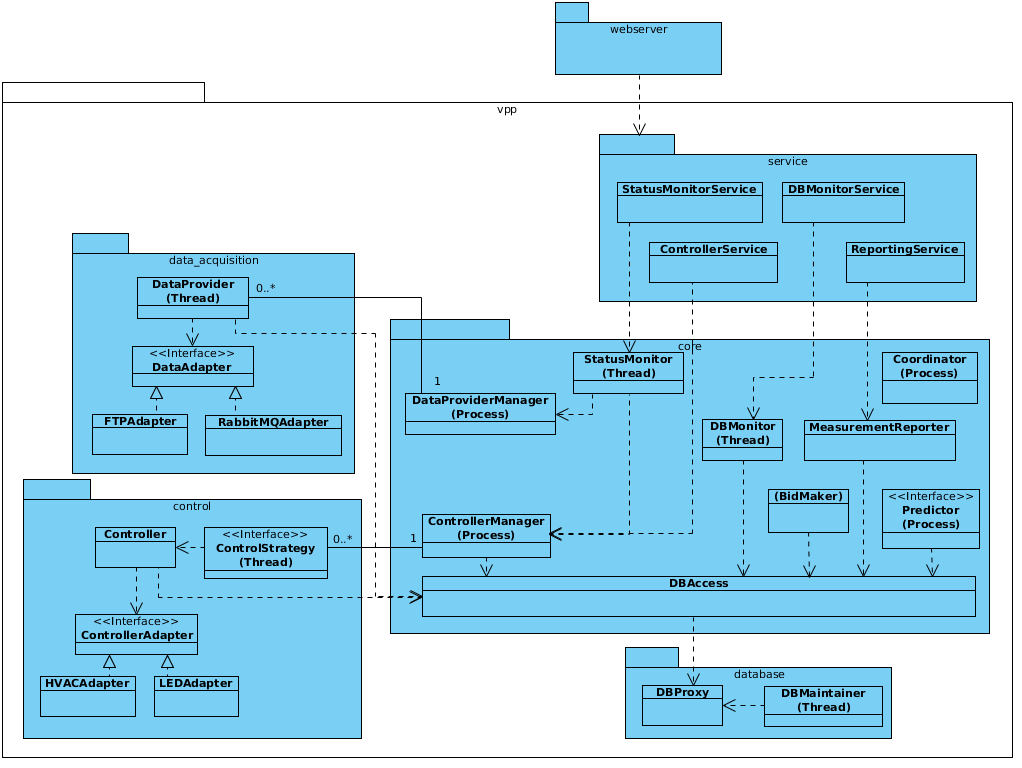
\includegraphics[width=\textwidth]{figures/class_diagram}
    \caption{Class diagram}
    \label{figureClassDiagram}
\end{figure}




%\begin{appendices}


\end{appendices}



\end{document}